\documentclass[german,10pt]{book}     
\usepackage{makeidx}
\usepackage{babel}            % Sprachunterstuetzung
\usepackage{amsmath}          % AMS "Grundpaket"
\usepackage{amssymb,amsfonts,amsthm,amscd} 
\usepackage{mathrsfs}
\usepackage{rotating}
\usepackage{sidecap}
\usepackage{graphicx}
\usepackage{color}
\usepackage{fancybox}
\usepackage{tikz}
\usetikzlibrary{arrows,snakes,backgrounds}
\usepackage{hyperref}
\hypersetup{colorlinks=true,
                    linkcolor=blue,
                    filecolor=magenta,
                    urlcolor=cyan,
                    pdftitle={Overleaf Example},
                    pdfpagemode=FullScreen,}
%\newcommand{\hyperref}[1]{\ref{#1}}
%
\definecolor{Gray}{gray}{0.80}
\DeclareMathSymbol{,}{\mathord}{letters}{"3B}
%
\newcounter{num}
\renewcommand{\thenum}{\arabic{num}}
\newenvironment{anmerkungen}
   {\begin{list}{(\thenum)}{%
   \usecounter{num}%
   \leftmargin0pt
   \itemindent5pt
   \topsep0pt
   \labelwidth0pt}%
   }{\end{list}}
%
\renewcommand{\arraystretch}{1.15}                % in Formeln und Tabellen   
\renewcommand{\baselinestretch}{1.15}                 % 1.15 facher
                                                      % Zeilenabst.
\newcommand{\Anmerkung}[1]{{\begin{footnotesize}#1 \end{footnotesize}}\\[0.2cm]}
\newcommand{\comment}[1]{}
\setlength{\parindent}{0em}           % Nicht einruecken am Anfang der Zeile 

\setlength{\textwidth}{15.4cm}
\setlength{\textheight}{23.0cm}
\setlength{\oddsidemargin}{1.0mm} 
\setlength{\evensidemargin}{-6.5mm}
\setlength{\topmargin}{-10mm} 
\setlength{\headheight}{0mm}
\newcommand{\identity}{{\bf 1}}
%
\newcommand{\vs}{\vspace{0.3cm}}
\newcommand{\noi}{\noindent}
\newcommand{\leer}{}

\newcommand{\engl}[1]{[\textit{#1}]}
\parindent 1.2cm
\sloppy

             \begin{document}  \setcounter{chapter}{1}

\chapter{SRT - Geometrische Konstruktionen}   %  Kap. 2
\label{chap_Geometrie}

In Kapitel \ref{chap_Grundlagen} wurden die Lorentz-Transformationen
aus den Axiomen der Speziellen Relativit\"atstheorie auf algebraischen Weg 
hergeleitet. In diesem Kapitel sollen die wesentlichen Eigenschaften dieser
Transformationen sowie insbesondere die Gleichzeitigkeitsfl\"achen und die
Hyperboloide zu gleichen Zeitdauern bzw.\ gleichen r\"aumlichen Abst\"anden
nochmals geometrisch hergeleitet werden. Die Einstein-Minkowski'sche Interpretation
der Speziellen Relativit\"atstheorie versteht die Lorentz-Invarianz der Theorie
als eine geometrische Eigenschaft der Raumzeit, aus der dann die Effekte
der Speziellen Relativit\"atstheorie abgeleitet werden k\"onnen. 

Die zugrundeliegenden Axiome bzw.\ Postulate der Speziellen Relativit\"tstheorie
sind:
begin{enumerate}
\item
Der Raum ist homogen und isotrop.
\item
Es gilt das Relativit\"atsprinzip.
\item
Die Konstanz der Lichtgeschwindigkeit ist unabh\"angig vom
Bewegungszustand der Lichtquelle.
\end{enumerate}
Diese drei Postulate werden im Folgenden genutzt, um die geometrischen Eigenschaften
der Raumzeit herzuleiten. 

\section{Der Raum gleichzeitiger Ereignisse}

Wir beginnen mit der geometrischen Konstruktion der Ereignismengen, die nach den
Axiomen der speziellen Relativit\"atstheorie von einem gegebenen Inertialsystem als gleichzeitig 
eingestuft werden. In einem vierdimensionalen Minkowski-Raum handelt es sich dabei um dreidimensionale
affine Unterr\"aume. In einer zweidimensionalen Darstellung handelt es sich um Geraden.

\begin{figure}[ht]
\setlength{\unitlength}{1.4pt}
\begin{picture}(153,120)(0,0)
\put(5,35){\vector(1,0){145}}
\put(65,5){\vector(0,1){110}}
\put(10,74){\line(1,0){120}}
\put(65,74){\makebox(0,0){{\footnotesize $\bullet$}}}
\put(26,74){\makebox(0,0){{\footnotesize $\bullet$}}}
\put(104,74){\makebox(0,0){{\footnotesize $\bullet$}}}
\put(65,35){\makebox(0,0){{\footnotesize $\bullet$}}}
\put(60,80){\makebox(0,0){$B$}}
\put(30,80){\makebox(0,0){$A$}}
\put(103,80){\makebox(0,0){$C$}}
\put(71,31){\makebox(0,0){$O$}}
\put(149,29){\makebox(0,0){$x$}}
\put(50,110){\makebox(0,0){$x^0=ct$}}
\put(68,100){\makebox(0,0){1}}
\thicklines
\put(35,5){\line(1,1){100}}
\put(95,5){\line(-1,1){86}}
\end{picture}
%
\begin{picture}(150,120)(0,0)
\put(55,5){\vector(1,3){36}}
\put(75,65){\makebox(0,0){{\footnotesize $\bullet$}}}
\put(45,55){\makebox(0,0){{\footnotesize $\bullet$}}}
\put(105,75){\makebox(0,0){{\footnotesize $\bullet$}}}
\put(65,35){\makebox(0,0){{\footnotesize $\bullet$}}}
\put(46,61){\makebox(0,0){$A'$}}
\put(71,69){\makebox(0,0){$B'$}}
\put(101,78){\makebox(0,0){$C'$}}
\put(71,31){\makebox(0,0){$O$}}
\put(15,45){\line(3,1){130}}
\put(6,15){\vector(3,1){144}}
\put(149,58){\makebox(0,0){$x'$}}
\put(107,110){\makebox(0,0){$x^{0\,\prime}=ct'$}}
\put(87,90){\makebox(0,0){2}}
\thicklines
\put(35,5){\line(1,1){100}}
\put(95,5){\line(-1,1){86}}
\end{picture}
\caption{\label{fig_gleichzeitig}%
Die gleichzeitigen Ereignisse f\"ur einen ruhenden
(links, Weltlinie 1) und einen relativ dazu bewegten 
Beobachter (rechts, Weltlinie 2) ergeben
sich aus der Forderung, dass f\"ur beide der Lichtkegel
zentriert ist, d.h.\ die Distanz $AB$ ($A'B'$) 
muss gleich der Distanz $BC$ ($B'C'$) sein.
Diese Bedingung legt in beiden F\"allen 
die Linie ABC (bzw.\ $A'B'C'$) 
eindeutig fest. Die Ereignisse auf dazu 
parallelen Linien (beispielsweise durch den Ursprung) 
sind f\"ur die Beobachter jeweils gleichzeitig.}
\end{figure}

Abbildung \ref{fig_gleichzeitig} zeigt zwei zweidimensionale
Raumzeit-Diagramme mit den Weltlinien zweier Beobachter
in verschiedenen Inertialsystemen.
Die Weltlinie von Beobachter 1 verlaufe entlang 
der $t$-Achse (mit der Raumkoordinate $x\equiv 0$),
die von Beobachter 2 entlang der $t'$-Achse (mit 
$x'\equiv 0$). Beide Beobachter haben bei
Ereignis O ihre Uhren auf $0$ gesetzt. Au\ss erdem 
hat es bei Ereignis O einen Lichtblitz gegeben, 
der sich entlang der Diagonalen
ausbreitet. Diese Diagonalen bilden den Zukunftslichtkegel
zum Ereignis O. (In Abbildung \ref{fig_gleichzeitig} sind auch
Teile des Vergangenheitslichtkegels zu O dargestellt.)

F\"ur beide Beobachter soll sich das Licht
in ihrem jeweiligen Inertialsystem in Vor- und
R\"uckrichtung gleich schnell ausbreiten.
Das bedeutet, zu dem Ereignis $B$ (bzw.\ $B'$) sind
auf dem Lichtkegel die Ereignisse $A$ und $C$
(bzw.\ $A'$ und $C'$) gleichzeitig, da nur f\"ur diese 
Ereignisse der Abstand AB und der Abstand BC 
(bzw.\ $A'B'$ und $B'C'$) gleich sind.
Offensichtlich sind die Ereignisse $A',B',C'$
f\"ur Beobachter 1 nicht gleichzeitig, umgekehrt
die Ereignisse $A,B,C$ nicht f\"ur Beobachter 2.

\section{Die Einstein-Synchronisation und Lichtuhren}

Auf dem genannten Verfahren beruht auch die
Einstein-Synchronisation von Uhren. Da nach Axiom
3 das Licht f\"ur jedes Inertialsystem in alle Richtungen 
dieselbe Ausbreitungsgeschwindigkeit hat, k\"onnen zwei
entferne Beobachter in konstantem Abstand 
(beide bewegen sich auf parallelen Weltlinien)
ihre Uhren dadurch synchronisieren, dass sie
ein Lichtsignal austauschen (vgl.\ Abb.\ \ref{fig_ES}): 
Beobachter 1 sendet
bei Ereignis A das Signal zu Beobachter 2, der es 
sofort reflektiert (Ereignis B) und zu Beobachter 1 
zur\"uckschickt, der es bei Ereignis C empf\"angt.
Beobachter 1 kann nun davon ausgehen, dass
das Licht f\"ur Hin- und R\"uckweg dieselbe Zeit
braucht. Bei der H\"alfte dieser Zeit sollte die
Uhr von Beobachter 1 also dieselbe 
Zeit angezeigt haben (Ereignis D), wie die
Uhr von Beobachter 2 bei Ereignis B.  

\begin{SCfigure}[50][htb]
\setlength{\unitlength}{1.7pt}
\begin{picture}(125,95)(-10,0)
\put(40,0){\vector(1,3){31}}
\put(13.5,0){\vector(1,3){31}}
\put(66.5,0){\vector(1,3){31}}
\put(55,45){\makebox(0,0){{\footnotesize $\bullet$}}}
\put(65,75){\makebox(0,0){{\footnotesize $\bullet$}}}
\put(25,35){\makebox(0,0){{\footnotesize $\bullet$}}}
\put(85,55){\makebox(0,0){{\footnotesize $\bullet$}}}
\put(45,15){\makebox(0,0){{\footnotesize $\bullet$}}}
\put(20,30){\makebox(0,0){B${}'$}}
\put(58,42){\makebox(0,0){D}}
\put(89,52){\makebox(0,0){B}}
\put(69,76){\makebox(0,0){C}}
\put(50,15){\makebox(0,0){A}}
\put(1,27){\line(3,1){109}}
%\put(169,98){\makebox(0,0){$x'$}}
\put(73,90){\makebox(0,0){1}}
\put(47,90){\makebox(0,0){3}}
\put(100,90){\makebox(0,0){2}}
\thicklines
\put(45,15){\line(1,1){65}}
\put(45,15){\line(-1,1){40}}
\put(85,55){\line(-1,1){20}}
\put(25,35){\line(1,1){40}}
%\put(30,20){\line(1,1){130}}
%\put(140,20){\line(-1,1){130}}
\end{picture}
\caption{\label{fig_ES}%
Die Einstein-Synchroni\-sation. Durch 
Austausch von Lichtsignalen k\"onnen die
Beobachter 2 und 3 ihre Uhren mit
der von Beobachter 1 synchronisieren.}
\end{SCfigure}

Das gleiche Verfahren erlaubt auch
eine Synchronisation der Uhren in
umgekehrter Richtung zwischen
Beobachter 1 und 3 und f\"uhrt auf
Ereignis $B'$, das zu Ereignis $D$
gleichzeitig ist. Man beachte, dass
die gleichzeitigen Ereignisse $B'$, 
$D$ und $B$ auf einer Geraden liegen.


\section{Die relativen Skalen in verschiedenen Inertialsystemen}

Wir m\"ussen noch die relativen Skalen festlegen. 
Dazu verlegen wir die beiden Koordinatensysteme
in dasselbe Bild (Abb.\ \ref{fig_scale}). Au\ss erdem
stellen wir uns die Abbildung senkrecht zur
Papierebene in eine zweite Raumdimension erweitert
vor: Den Lichtkegel erh\"alt man durch Rotation
um die $t$-Achse, die Gleichzeitigkeitsebenen
von Beobachter 1 durch Ereignis $B$ und von
Beobachter 2 durch Ereignis $B'$ stehen senkrecht
auf der Papierebene.  

\begin{figure}[ht]
\setlength{\unitlength}{2pt}
\begin{picture}(180,120)(0,0)
\put(10,35){\vector(1,0){160}}
\put(85,5){\vector(0,1){110}}
\put(70,5){\vector(1,2){53}}
\qbezier(19,102.5)(85,35)(151,102.5)
\put(103,71){\makebox(0,0){{\footnotesize $\bullet$}}}
\put(85,68.5){\makebox(0,0){{\footnotesize $\bullet$}}}
\put(66.5,53){\makebox(0,0){{\footnotesize $\bullet$}}}
\put(140,90){\makebox(0,0){{\footnotesize $\bullet$}}}
\put(85,35){\makebox(0,0){{\footnotesize $\bullet$}}}
\put(51.5,68.5){\makebox(0,0){{\footnotesize $\bullet$}}}
\put(118.5,68.5){\makebox(0,0){{\footnotesize $\bullet$}}}
\put(67,58){\makebox(0,0){$A'$}}
\put(100,75){\makebox(0,0){$B'$}}
\put(140,85){\makebox(0,0){$C'$}}
\put(82,73){\makebox(0,0){$B$}}
\put(91,32){\makebox(0,0){$O$}}
\put(51,64){\makebox(0,0){$A$}}
\put(119,64){\makebox(0,0){$C$}}
\put(34,37){\line(2,1){126}}
\put(40,68.5){\line(1,0){90}}
\put(31,8){\vector(2,1){130}}
\put(169,29){\makebox(0,0){$x$}}
\put(169,58){\makebox(0,0){$x'$}}
\put(81,110){\makebox(0,0){$t$}}
\put(118,108){\makebox(0,0){$t'$}}
\thicklines
\put(55,5){\line(1,1){100}}
\put(115,5){\line(-1,1){100}}
\end{picture}
\caption{\label{fig_scale}%
F\"ur Beobachter 1 sind die Ereignisse $A,B,C$ gleichzeitig,
f\"ur Beobachter 2 die Ereignisse $A',B',C'$. Der Einfachheit
halber wurde $c=1$ gesetzt (bzw.\ $t$ entspricht $x^0$). 
Daher ist die Strecke $OB$ gleich $AB$ bzw.\ $BC$.
Aus demselben Grund ist $OB'=A'B'=B'C'$.
Die Strecke $OB$ ist aber auch gleich $OB'$, da
das Licht in der Richtung senkrecht zur Papierebene
f\"ur diese beiden Ereignisse dieselbe Strecke
zur\"uckgelegt hat.}
\end{figure}
 
Die Ereignisse $A$ und $C$ geh\"oren in $(2+1)$-Raumzeitdimensionen
zu einem Kreis mit Zentrum $B$. Der Radius dieses Kreises
ist $AB=BC=OB$. Entsprechend geh\"oren die Ereignisse
$A'$ und $C'$ (in unserer euklidischen Geometrie) zu einer
Ellipse (der Schnittmenge des Kegels mit einer Ebene), 
in deren Zentrum sich $B'$ befindet. Die gro\ss e
Halbachse dieser Ellipse ist $A'B'=B'C'$. Nach unserer
Forderung, dass sich Licht in alle Richtungen mit derselben
Geschwindigkeit ausbreitet, hat diese gro\ss e Halbachse in
der Minkowski-Geometrie dieselbe L\"ange wie die kleine
Halbachse (senkrecht zu $B'$). Doch die Mittelpunkte aller 
Ellipsen, deren gro\ss e Halbachse in der Zeichenebene 
liegen und deren kleine Halbachsen dieselbe L\"ange
haben, liegen auf der Hyperbel $t^2 - x^2 = {\rm const}$
(dazu schneide man den Kegel einfach mit einer senkrechten
Ebene parallel zur Zeichenebene). Also ist in der Zeichnung
die Strecke $OB'$ gleich der Strecke $OB$, wodurch wir
auch die Skala festgelegt haben.

\begin{SCfigure}[50][ht]
\setlength{\unitlength}{1.7pt}
\begin{picture}(150,120)(10,0)
\put(100,5){\vector(-1,2){53}}
\put(85,5){\vector(0,1){110}}
\put(70,5){\vector(1,2){53}}
\put(62,5){\vector(3,4){78}}
\qbezier(19,102.5)(85,35)(151,102.5)
\put(103,71){\makebox(0,0){{\footnotesize $\bullet$}}}
\put(85,68.5){\makebox(0,0){{\footnotesize $\bullet$}}}
\put(115,76){\makebox(0,0){{\footnotesize $\bullet$}}}
\put(67,71){\makebox(0,0){{\footnotesize $\bullet$}}}
\put(85,35){\makebox(0,0){{\footnotesize $\bullet$}}}
\put(100,76){\makebox(0,0){$B_2$}}
\put(113,81){\makebox(0,0){$B_3$}}
\put(81,73){\makebox(0,0){$B_1$}}
\put(91,35){\makebox(0,0){$O$}}
\put(70,76){\makebox(0,0){$B_4$}}
\put(88,55){\makebox(0,0){$\tau$}}
\put(135,110){\makebox(0,0){$t_3$}}
\put(81,110){\makebox(0,0){$t_1$}}
\put(118,110){\makebox(0,0){$t_2$}}
\put(52,110){\makebox(0,0){$t_4$}}
\thicklines
\put(55,5){\line(1,1){100}}
\put(115,5){\line(-1,1){100}}
\end{picture}
\caption{\label{fig_hyperbel}%
F\"ur alle inertialen Weltlinien durch
das Ereignis $O$ ist bei den Ereignissen
$B_i$ auf der Hyperbel dieselbe 
Zeit vergangen: Alle Uhren entlang 
dieser Weltlinien, die bei $O$ auf 0
gesetzt wurden, zeigen bei den
Ereignissen $B_i$ dieselbe Zeit $\tau$
an.}
\end{SCfigure}

Nachdem wir die zeitlichen Skalen zu
verschieden \glqq geneigten\grqq\
Strecken gefunden haben, k\"onnen wir
auch die entsprechenden r\"aumlichen
Skalen konstruieren. Wegen der
Konstanz der Lichtausbreitung in allen
Systemen hatten wir in Abb.\ \ref{fig_scale}
argumentieren k\"onnen, dass die 
zeitliche Distanz $OB'$ gleich der
r\"aumlichen Distanz $B'C'$ (jeweils
als positive Werte aufgefasst) sein
muss. Damit k\"onnen wir aus
Abb.\ \ref{fig_hyperbel} auf
Abb.\ \ref{fig_laengen} schlie\ss en
und feststellen, dass alle
zu $O$ raumartigen Ereignisse 
$A_i$ von $O$ dieselbe 
Entfernung haben.

\begin{SCfigure}[50][ht]
\setlength{\unitlength}{1.7pt}
\begin{picture}(120,140)(0,0)
\put(5,85){\vector(2,-1){110}}
\put(5,70){\vector(1,0){110}}
\put(5,55){\vector(2,1){110}}
\put(5,47){\vector(4,3){110}}
\qbezier(103.5,4)(33.5,70)(103.5,136)
\put(71,88){\makebox(0,0){{\footnotesize $\bullet$}}}
\put(68.5,70){\makebox(0,0){{\footnotesize $\bullet$}}}
\put(76,100){\makebox(0,0){{\footnotesize $\bullet$}}}
\put(71,52){\makebox(0,0){{\footnotesize $\bullet$}}}
\put(35,70){\makebox(0,0){{\footnotesize $\bullet$}}}
\put(75,86){\makebox(0,0){$A_2$}}
\put(80,99){\makebox(0,0){$A_3$}}
\put(73,66){\makebox(0,0){$A_1$}}
\put(35,76){\makebox(0,0){$O$}}
\put(76,55){\makebox(0,0){$A_4$}}
\put(55,74){\makebox(0,0){$L$}}
\put(110,120){\makebox(0,0){$x_3$}}
\put(110,66){\makebox(0,0){$x_1$}}
\put(110,103){\makebox(0,0){$x_2$}}
\put(110,37){\makebox(0,0){$x_4$}}
\thicklines
\put(5,40){\line(1,1){100}}
\put(5,100){\line(1,-1){100}}
\end{picture}
\caption{\label{fig_laengen}%
Alle Ereignisse $A_i$ haben von $O$
denselben invarianten r\"aumlichen
Abstand $L$. Das bedeutet, zu jedem 
Ereignis $A_i$ gibt es ein Inertialsystem,
sodass $O$ und $A_i$ gleichzeitig
stattfinden. Die r\"aumliche Differenz in
diesem Inertialsystem ist gleich dem
invianten r\"aumlichen Abstand der Ereignisse.}
\end{SCfigure}


\begin{figure}[htbp]
%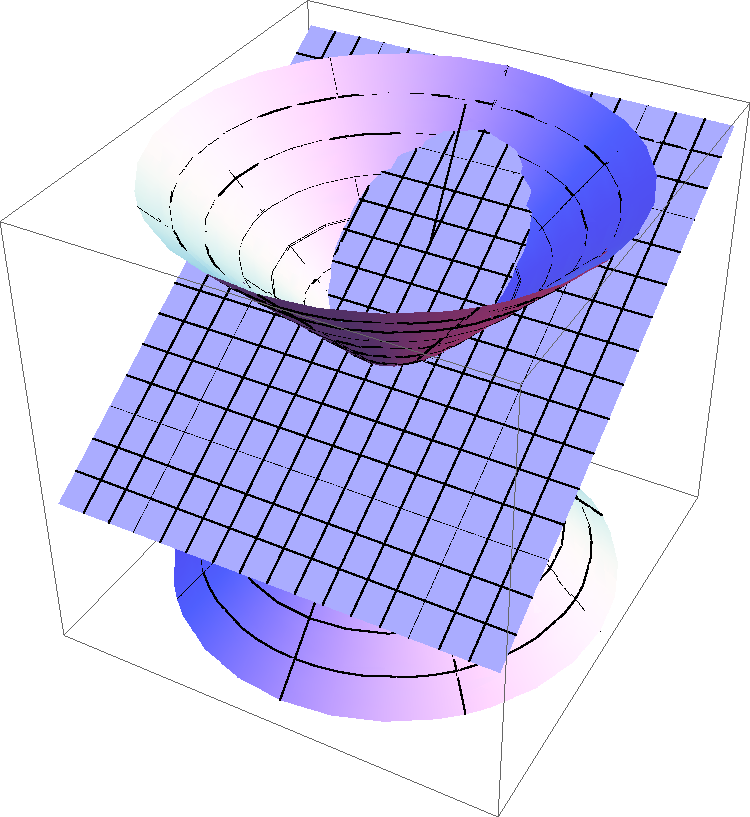
\includegraphics[width=0.47\linewidth,height=0.45\linewidth,clip]{Lightcone_2} %\hspace{0.3cm}
%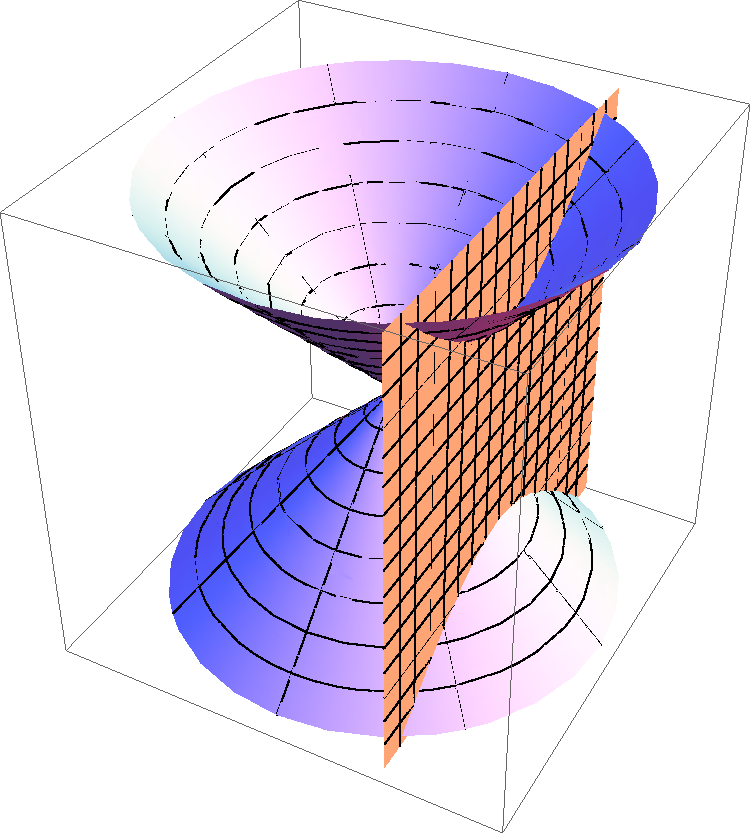
\includegraphics[width=0.5\linewidth,height=0.5\linewidth,clip]{Lightcone_1}
\caption[]{ \label{fig:lightcone}
(links) In zwei Raumdimensionen schneidet die Gleichzeitigkeitsebene
zu einem Beobachter 2 den Lichtkegel in einer Ellipse. Die
gro\ss e Halbachse entspricht dem gesuchten Abstand $A'B'$ 
bzw.\ $B'C'$, die kleine Halbachse ist senkrecht zur
relativen Bewegung und hat daher f\"ur Beobachter 1 und
2 dieselbe L\"ange. Andererseits soll sich f\"ur Beobachter
2 das Licht in alle Richtungen gleich schnell ausbreiten, d.h.\
f\"ur Beobachter 2 haben die gro\ss e und die kleine
Halbachse der Ellipse dieselbe L\"ange. (rechts)
Die Punkte mit einem konstanten Abstand von der
$(x,t)$-Ebene schneiden den Lichtkegel in einer
Hyperbel, d.h.\ alle Punkte auf dieser Hyperbel haben 
von der $(x,t)$-Ebene denselben Abstand.}
\end{figure}


Wir haben oben die relative Skala durch Vergleich mit
einer zweiten Raumdimension, relativ zu der sich zwei
Inertialsysteme nicht bewegen, abgeleitet. Es gibt noch eine
zweite M\"oglichkeit, die sich auch in zwei Dimensionen 
anwenden l\"asst:
Wir integrieren das Vektorfeld, das in jedem Punkt durch
die Richtung der Gleichzeitigkeit erzeugt wird. Dies f\"uhrt auf die
Bedingung\index{Gleichzeitigkeit}
\[    \frac{{\rm d}x}{{\rm d}t} ~=~ \frac{t}{x} 
      \hspace{1cm} {\rm oder} \hspace{1cm}
      t^2 - x^2 ~=~ {\rm const.}~~  . \]
Alle Ereignisse auf einer solchen Hyperbel haben denselben 
Abstand vom Ursprung. Insbesondere gilt
\[    t_{\rm B}^2 - x_{\rm B}^2 ~=~ t_{\rm D}^2  \;, \]
und da $x_{\rm B} =v t_{\rm B}$ folgt
\[    t_{\rm B}^2 - v^2 t_{\rm B}^2 ~=~ t_{\rm D}^2 \]
oder 
\[       t_{\rm D} ~=~ \frac{1}{\sqrt{1-v^2}} t_{\rm B}  \;. \]
Dieses Verfahren setzt voraus, dass Ereignisse mit einem konstanten
Abstand vom Ursprung in gewisser Hinsicht \glqq stetig\grqq\ sind, und da\ss\
wir infinitesimal annehmen k\"onnen, dass solche Ereignisse f\"ur
einen Beobachter, der sich gleichf\"ormig vom Ursprung zu einem dieser
Ereignisse bewegt, lokal gleichzeitig sind.



\begin{thebibliography}{99}
\addcontentsline{toc}{chapter}{Literaturangaben}
\bibitem{Aichelburg} Peter C.\ Aichelburg (Hrsg.); {\it Zeit im 
       Wandel der Zeit}; Verlag Vieweg, Braunschweig, Wiesbaden, 1988.
\bibitem{Born} Max Born; {\it Optik}; Springer-Verlag, Berlin, Heidelberg,
        1972.
\bibitem{Britannica} Encyclopaedia Britannica; 15.th edition, 1988.
\bibitem{Descartes} Ren\'e Descartes; {\it Die Prinzipien der
        Philosophie}; Felix Meiner Verlag, Hamburg, 1992; \"ubersetzt
        von Artur Buchenau.
\bibitem{Einstein1} Albert Einstein; {\it Zur Elektrodynamik bewegter 
        K\"orper}; Annalen der Physik, Leipzig, 17 (1905) 891. 
\bibitem{Helmholtz2} Hermann von Helmholtz; {\em \"Uber Wirbelbewegungen,
        \"Uber Fl\"ussigkeitsbewegungen}, 1858; in Ostwalds Klassiker der 
       exakten Wissenschaften Bd.\ 1; Verlag Harri Deutsch, Frankfurt, 
       1996.                   
\bibitem{Laue} Max von Laue; {\it Geschichte der Physik}; 
         Universit\"ats-Verlag Bonn, 1947.
\bibitem{Lorentz} Hendrik Antoon Lorentz; {\it Electromagnetic phenomena 
         in a system moving with any velocity smaller than that of light}; 
         Proc.\ Acad.\ Sci., Amsterdam, 6 [1904], S.\ 809.
\bibitem{Mittelstaedt} Peter Mittelstaedt; {\it Der Zeitbegriff in der
        Physik}; BI-Wissenschaftsverlag, 1989.        
\bibitem{Mittelstaedt2} Peter Mittelstaedt; {\it Philosophische Probleme
        der modernen Physik}; BI-Wissenschaftsverlag, 1989.        
\bibitem{Newton2} Isaac Newton; {\it \"Uber die Gravitation...};
       Klostermann Texte Philosophie; Vittorio Klostermann, Frankfurt,
      1988; \"ubersetzt von Gernot B\"ohme.
\bibitem{Newton3} Isaac Newton; {\it Optik oder Abhandlung \"uber
      Spiegelungen, Brechungen, Beugungen und Farben des Lichts};
      I., II.\ und III.\ Buch (1704); aus dem Englischen \"ubersetzt
      von W.\ Abendroth; Ostwalds Klassiker der exakten Wissenschaften,
      Verlag Harri Deutsch 1998.   
\bibitem{Pauli} Wolfgang Pauli; {\it Theory of Relativity}; Dover
      Publications, New York, 1981.      
\bibitem{Poincare} Jules Henri Poincar\'e; {\it Sur la dynamique de 
     l'\'electron}, C.R.\ Acad.\ Sci., Paris, 140 (1905) S.~1504; und 
      Rendiconti del Circolo Matematico di Palermo, Bd.~21 (1906) S.~129.
\bibitem{Sexl} Roman U.\ Sexl, Helmuth K.\ Urbantke; {\it Relativit\"at,
      Gruppen, Teilchen}; Springer-Verlag, Wien, New York, 1992.
\bibitem{Simonyi}
      K\'aroly Simonyi; {\it Kulturgeschichte der Physik}; Verlag
       Harri Deutsch, Thun, Frankfurt am Main, 1990.
\end{thebibliography}

\end{document}
